\section*{Aufgabe 2}

\begin{enumerate}[label=\alph*)]
    \item 
    Es ist 
    \begin{align*}
        R &= \sum_i (mx_i+n-y_i)^2
        =
        \begin{pmatrix}
            mx_0 + n - y_0 \\
            mx_1 + n - y_1 \\
            \vdots\\
            mx_n + n - y_n \\
        \end{pmatrix}^2
        =
        \left(
        \underbrace{
        \begin{pmatrix}
            x_0 & 1 \\
            x_1 & 1 \\
            \vdots & \vdots \\
            x_n & 1
        \end{pmatrix}}_{\tilde M}
        \cdot
        \underbrace{
        \begin{pmatrix}
            m\\n
        \end{pmatrix}}_{\vec a}
        - 
        \underbrace{
        \begin{pmatrix}
            y_0 \\ y_1 \\ \vdots \\ y_n
        \end{pmatrix}}_{\vec y}\right)^2\\
        &= (\tilde M\vec a - \vec y)^2
        = (\tilde M\vec a - \vec y)^T\cdot (\tilde M\vec a - \vec y).
    \end{align*}
    
    
    Der Vektor $\vec a$ soll nun so eingestellt werden, dass $R$ minimal wird.
    Liegen die Punkte genau auf einer Geraden, so kann da Problem exakt gelöst werden und die Lösung des überbestimmten Gleichungssystems ist
    $\tilde M \vec a - \vec y$, wobei $R=0$ ist.
    \item
    Ist das überbestimmte Problem nicht zu lösen, 
    so lässt sich jedoch $R$ durch die Lösung eines quadratischen Gleichungssystems minimieren, dazu muss:
    \begin{align*}
        \frac{\partial R}{\partial \vec a}
        &=
        2 (\tilde M\vec a - \vec y)^T \tilde M
        = 2 (\tilde M^T\tilde M\vec a - \tilde M^T\vec y)^T
        \overset{!}{=} 0\\
        &\Rightarrow 
        \tilde M^T\tilde M\vec a - \tilde M^T\vec y = 0
        \Leftrightarrow 
        \underbrace{\tilde M^T\tilde M\vec a = \tilde M^T\vec y}_{
            \text{Quadr. LGS}
        }
    \end{align*}
     Dieses System kann nun numerisch gelöst werden.
    
    \item Das Problem wird numerisch analog zu Aufgabe 1 gelöst. Der Lösungsvektor ergibt sich zu 
    \begin{equation*}
        \vec a = \begin{pmatrix}
            \num{0.96}\\
            \num{2.66}\\
        \end{pmatrix}.
    \end{equation*}

    \item   Die Datenpunkte und die Ausgleichsgerade sind in Abb. \ref{fig:ausgleich} graphisch dargestellt.
            \begin{figure}
                \centering
                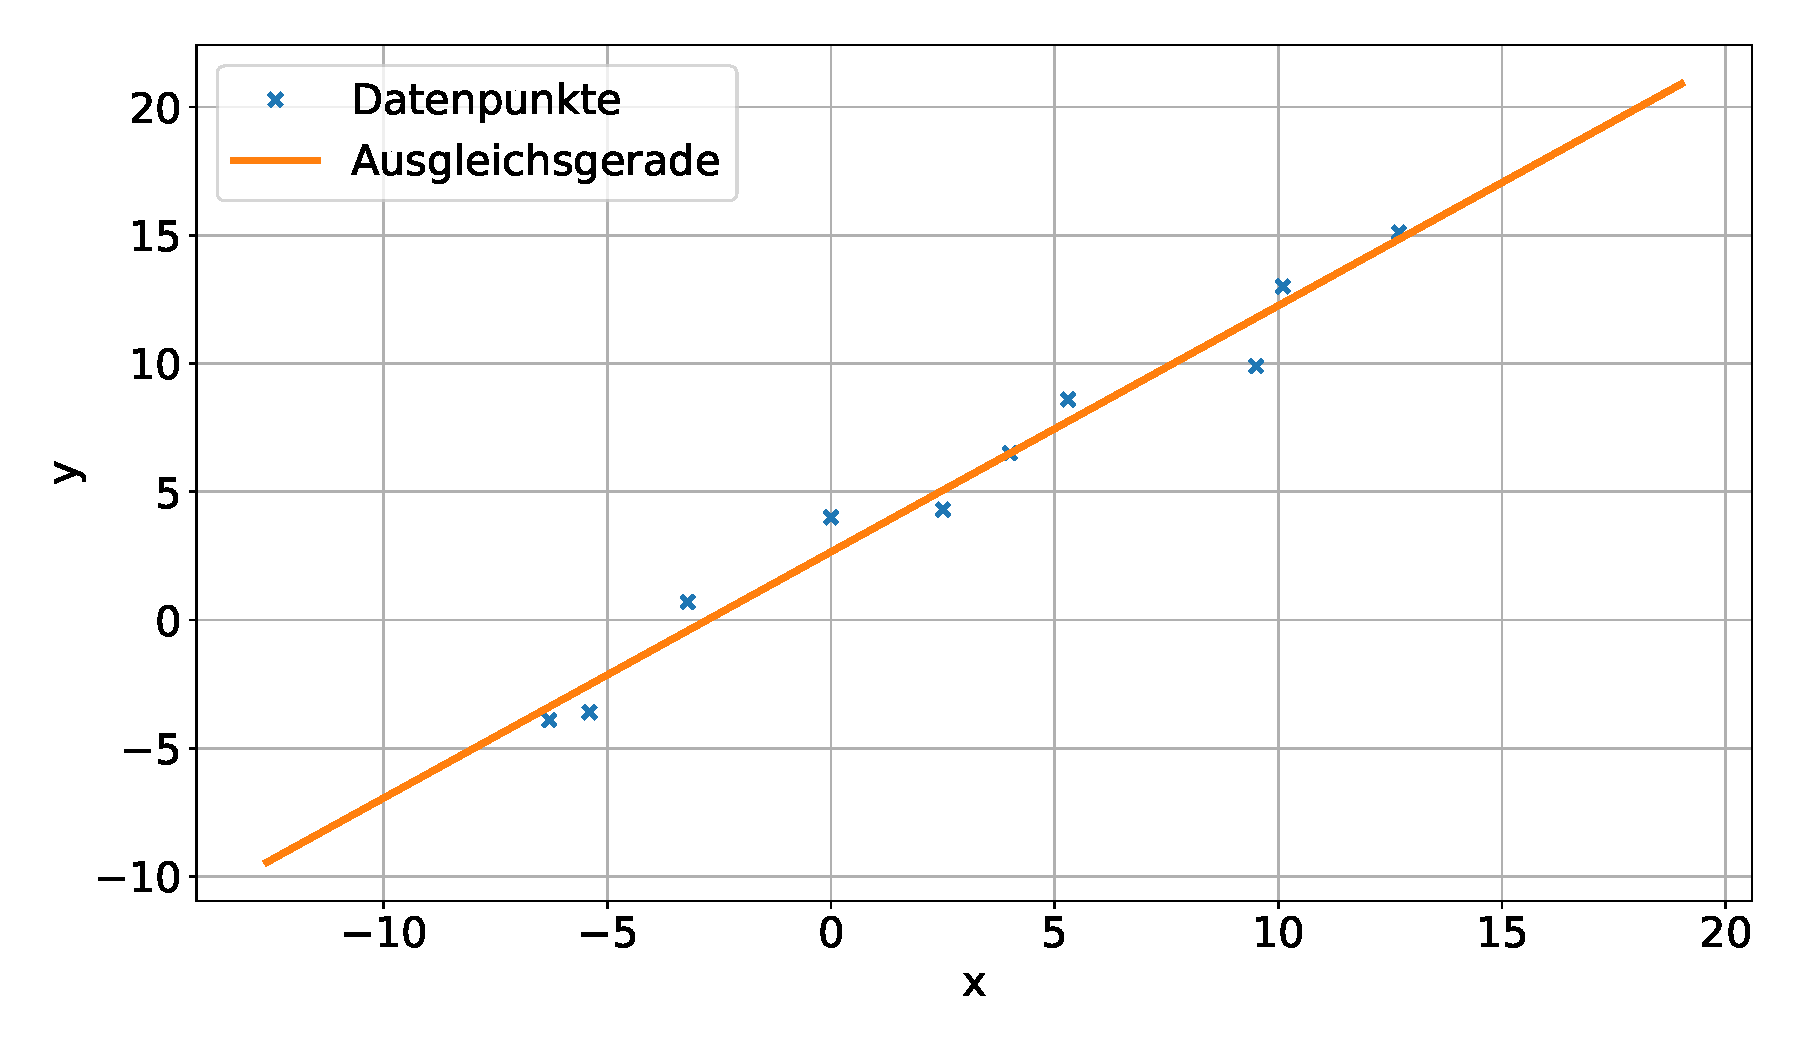
\includegraphics[width=0.8\textwidth]{./bin/figure.pdf}
            \caption{Das Ergebnis der Ausgleichsrechnung.}
            \label{fig:ausgleich}
            \end{figure}
\end{enumerate}